
\textbf{مورد استفاده:}
نمایش پروژه‌ها
\\
\textbf{شرح مختصر :UC}
نمایش لیست پروژه‌های فعال در سایت.
\\
\textbf{پيش شرط:}
ندارد.
\\
\textbf{سناريو اصلی:}
\begin{enumerate}
\item
شروع
\item
مهمان دکمه پروژه‌ها را انتخاب می‌کند و سیستم لیست کل پروژه‌ها را به مهمان نمایش می‌دهد.
\item
مهمان با انتخاب هر پروژه‌ها به اطلاعات آن دسترسی پیدا می‌کند.
\item
پایان
\end{enumerate}

\noindent
\textbf{پس شرط:}
ندارد.
\\
\textbf{سناريوهای فرعی:}
\\
ندارد.
\\
\textbf{پس شرط:}
ندارد.


\begin{figure}[H]
	\centering
	\includegraphics[width=.8\textwidth]{Diagram/2.Activity/لیست-پروژه‌ها.jpg}
	\caption{دیاگرام فعالیت لیست پروژه‌ها}
	\label{fig:a:لیست-پروژه‌ها}
\end{figure}
\begin{figure}[H]
	\centering
	%\includegraphics[width=1\textwidth]{Diagram/3.Sequence/لیست-پروژه‌ها.jpg}
	\caption{دیاگرام توالی لیست پروژه‌ها}
	\label{fig:s:لیست-پروژه‌ها}
\end{figure}
\begin{figure}[H]
	\centering
	%\includegraphics[width=1\textwidth]{Diagram/4.Collaboration/لیست-پروژه‌ها.jpg}
	\caption{دیاگرام همکار لیست پروژه‌ها}
	\label{fig:c:لیست-پروژه‌ها}
\end{figure}